\chapter{Introduction}

The emerging picture of the last century is that the elements described by the Periodic Table are themselves not the most fundamental forms found in Nature. We have learned that these elements are made of atoms consisting of bound states of protons, neutrons, and electrons. We have discovered that these protons and neutrons themselves are made of more fundamental components called quarks and gluons. And so as the Periodic Table before it, the Standard Model of particle physics (SM) seen in Figure~\ref{fig:sm}, has been developed to provide an organizing principle for what we currently understand to be the correct description for the strong and electroweak forces, describing the fundamental particles and forces that form the Universe (the SM does not address gravity). The discovery of the Higgs boson in 2012 \cite{higgsdisc} completed the search for all the fundamental particles addressed within the theory, a truly monumental achievement. As time goes on experimental verification only grows stronger.

\begin{figure}
\centering
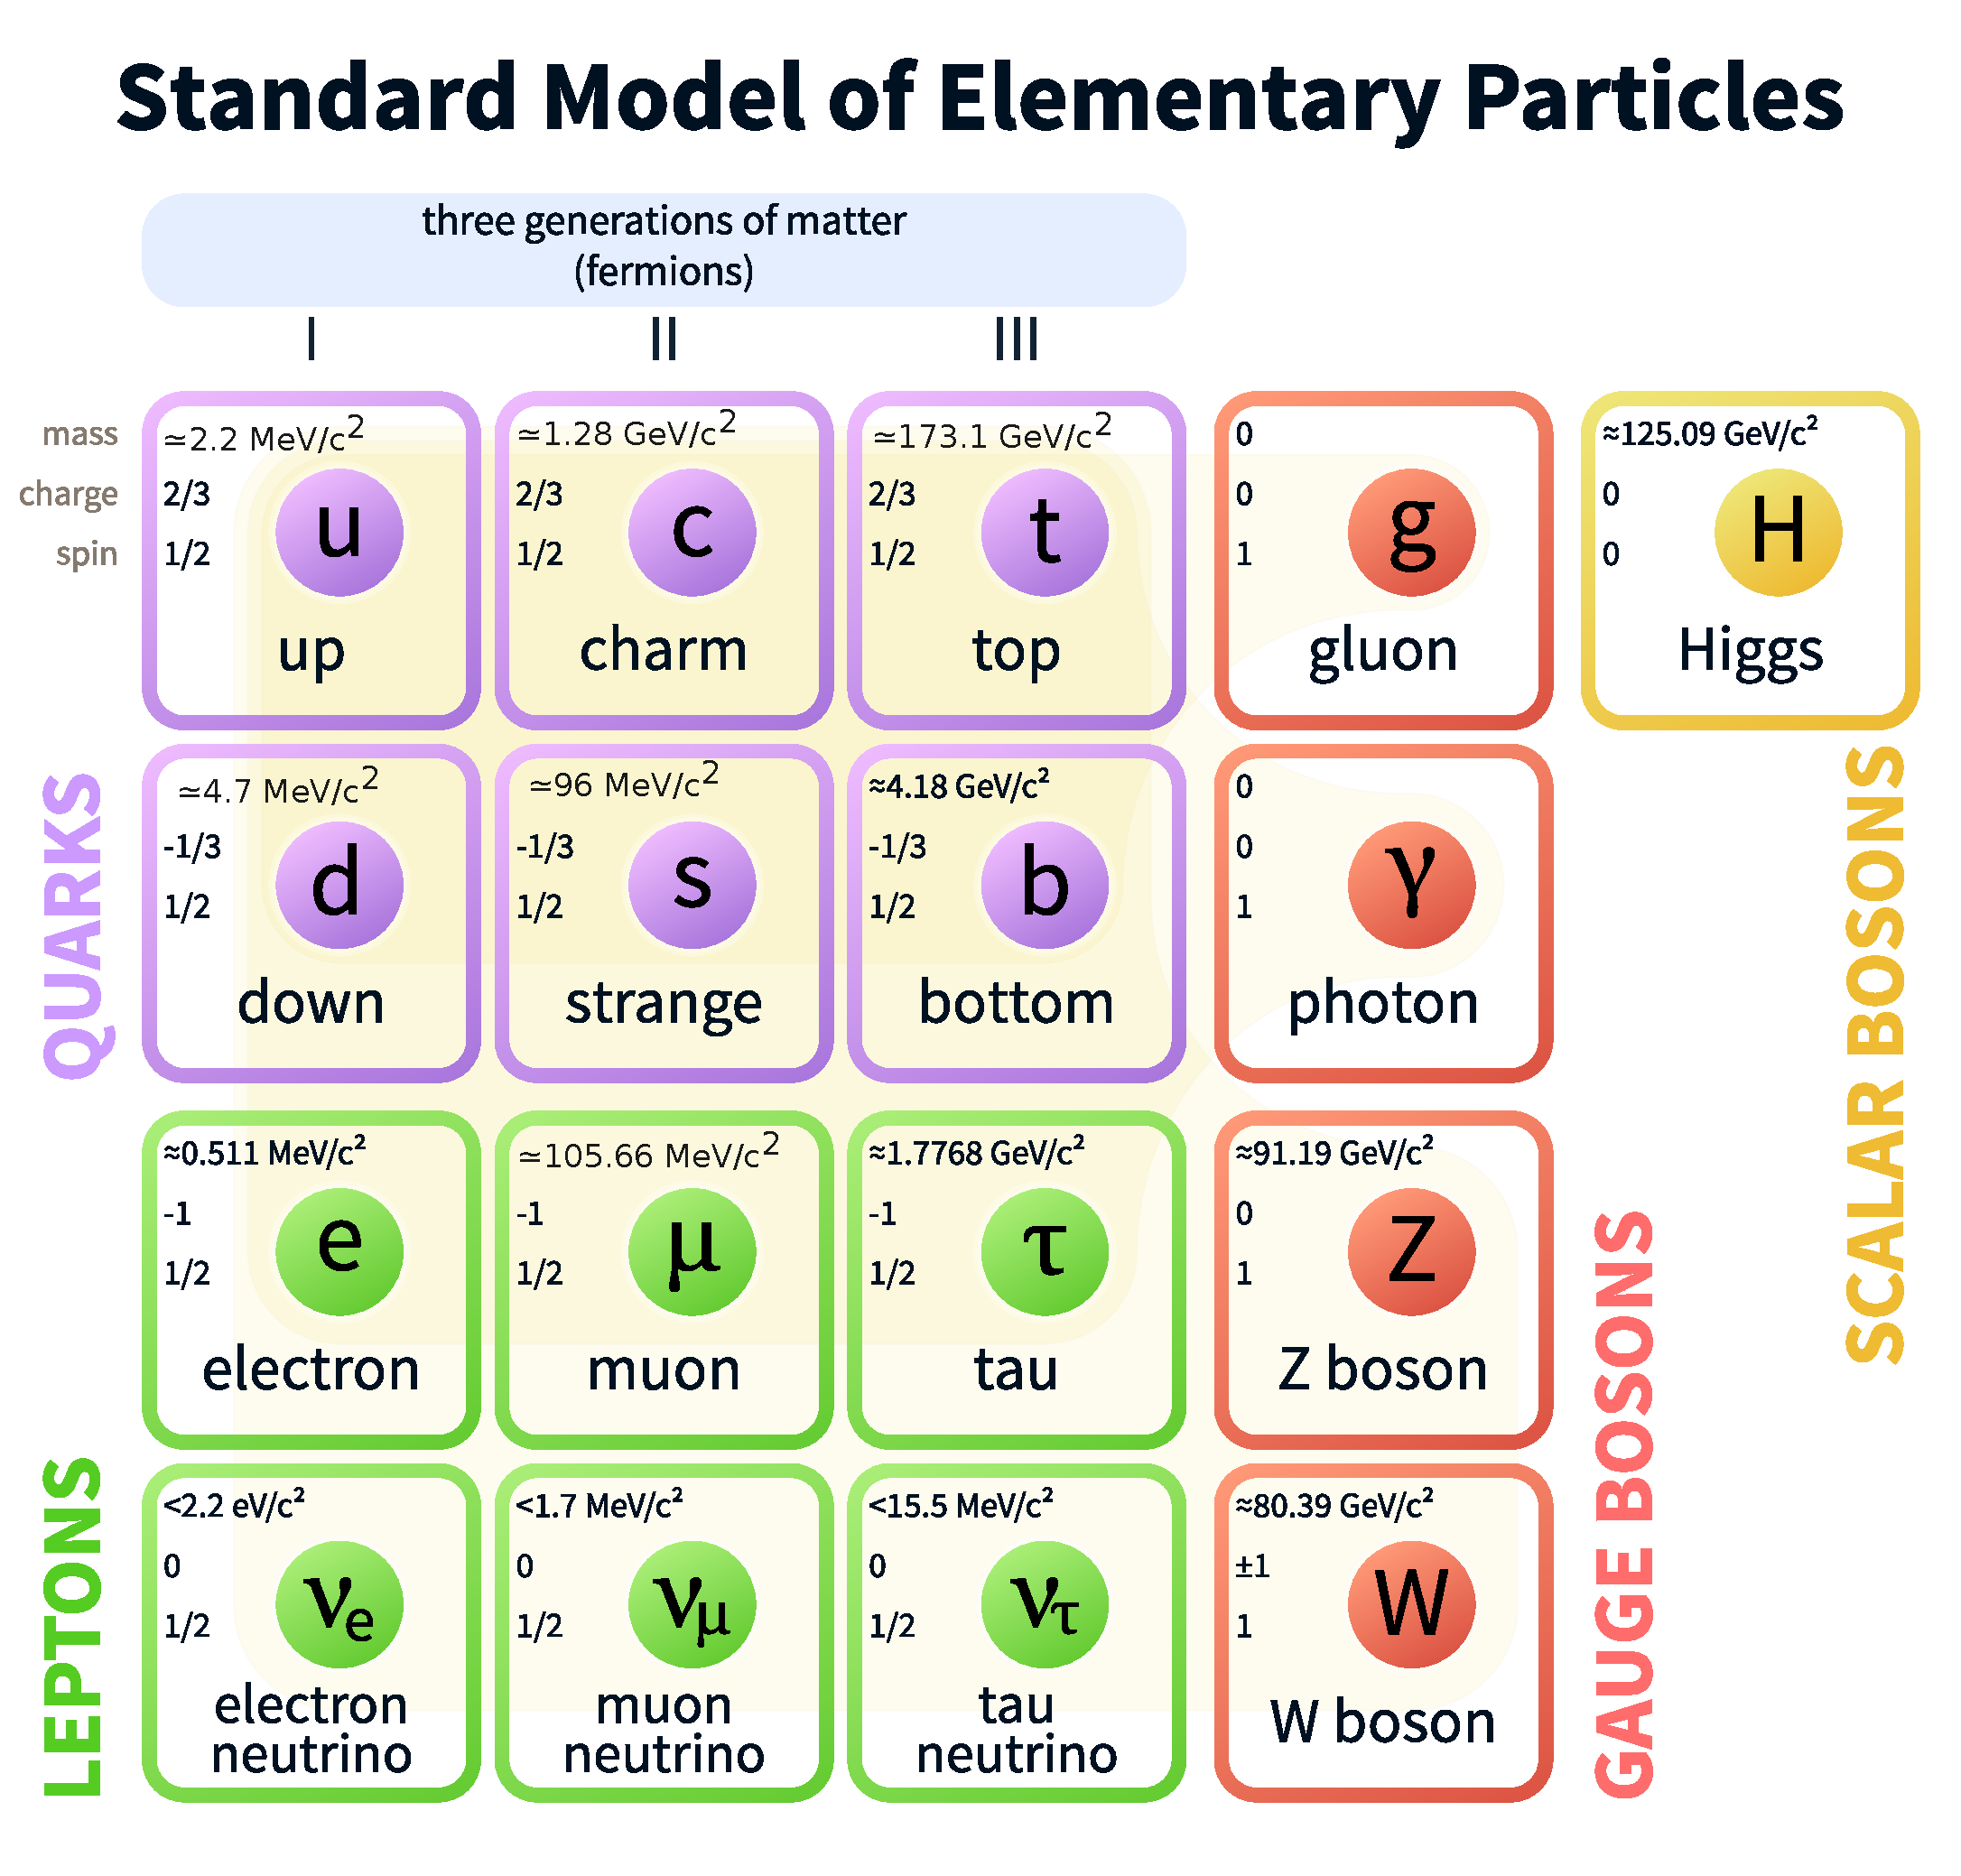
\includegraphics[width=0.8\textwidth]{figs/StandardModelofElementaryParticles.pdf}
\caption[The particles in the Standard Model of particle physics.]{The particles in the Standard Model of particle physics. \cite{wiki:xxx}}
\label{fig:sm}
\end{figure}

But, there are many both experimental and theoretical indications that the SM is not the final story. Cosmological observations require the presence of a ``dark matter'' in the Universe, a ubiquitous substance thought to account for 85\% of the total matter in the Universe. Although its influence has been observed in gravitational lensing phenomena and galaxy rotation curves, we do not yet have a particle description of its nature. One theoretical motivation that points toward the SM being a part of some grander theory is known as a ``fine-tuning'' problem. Because the Higgs boson is a scalar particle (the only such fundamental particle in the SM), its mass receives quantum mechanical corrections that are strongly dependent on the ultraviolet cutoff $\Lambda_{\textrm{UV}}$ or other high mass scales in the theory. As the most natural cutoff is likely at the Grand Unified Theory or Planck scale, we would expect the Higgs boson mass to be extremely large, many orders of magnitude larger than it has experimentally been determined to be. This implies that there is some sort of `unnatural' collusion between the correction terms, which is somehow able to bring the mass to the electroweak scale (this is known as a \textit{hierarchy problem}).

Supersymmetry (SUSY) is an elegant extension to the SM which is able to address many of these issues. In addition to the SU(3)xSU(2)xU(1) symmetries of the SM, SUSY introduces space-time symmetries relating fermionic and bosonic degrees of freedom. The particle content within the simplest of such SUSY models, the Minimal Supersymmetric SM (MSSM), is over twice that of the SM as each particle requires a "superpartner" differing by 1/2 unit of spin. The lightest neutral particle of the theory, expected to remain stable, is a popular candidate for particle dark matter. The addition of these superpartners to the theory yield quantum mechanical corrections to the Higgs mass that enter with the opposite sign and naturally are able to cancel the terms up to $\Lambda_{\textrm{UV}}$. An exact supersymmetry requires that these superpartners have identical mass to their SM counterpart. As we have not observed any such particles, it must be that the supersymmetry is broken, resulting in the partners acquiring large mass through some other means. These masses must be sufficiently large that small production cross sections at collider experiments have not allowed for their unambiguous detection. A major motivating force for the construction of the LHC is finding evidence of SUSY. The analysis presented in this thesis presents one such search, focusing in one small parameter space of the vast possibilities.

The thesis is outlined as follows: A description of the Standard Model (SM) of particle physics, the theory describing the known fundamental forces and particles, is presented in Chapter~\ref{chap:sm}. A description of the Minimal Supersymmetric Standard Model (MSSM), one extension to the SM able to provide answers to many of our questions, is presented in Chapter~\ref{chap:mssm}. A description of the Large Hadron Collider (LHC), the facility that acts as our source of high-energy proton-proton collisions, is presented in Chapter~\ref{chap:lhc}. A description of the CMS particle detector, responsible for the detection of particles and reconstruction of the proton interactions, is presented in Chapter~\ref{chap:detector}. A description of how the data from the detector are reconstructed and identified as physical particles is presented in Chapter~\ref{chap:eventreco}. The focus of the thesis, a description of how the physics data can be used to search for evidence of new particles such as those predicted by SUSY, is presented in Chapter~\ref{chap:analysis}. The conclusions are presented in Chapter~\ref{chap:conclusions}. Appendix~\ref{chap:bb} presents a more detailed discussion of the \bbbar-tagging algorithm used in this analysis. Appendix~\ref{chap:reinterpretation} provides tagging efficiencies for the reconstruction of Higgs and Z bosons relevant to the analysis. Appendix~\ref{chap:bbsf} presents a calculation of scale factors, correcting differences in simulation from data, for $b\bar{b}$-tagging W boson jets --- a topic partly independent from the rest of the thesis.
